\subsection{Κόσμος - Αντικείμενα}

Ο κόσμος του παιχνιδιού περιέχει λίγα και βασικά αντικείμενα με απλά χρώματα, κάτι το οποίο έχει ως στόχο την πλήρη συγκέντρωση του παίκτη στις τιμές και στον αλγόριθμο.

\subsubsection{Κουτιά τιμών}

Τα κουτιά, τα οποία περιέχουν τις τιμές, μπορούν να βρίσκονται σε τρεις διαφορετικές καταστάσεις: \textbf{άδειο}, \textbf{γεμάτο} και \textbf{κλειδωμένο}.

\begin{figure}[H]
    \centering
    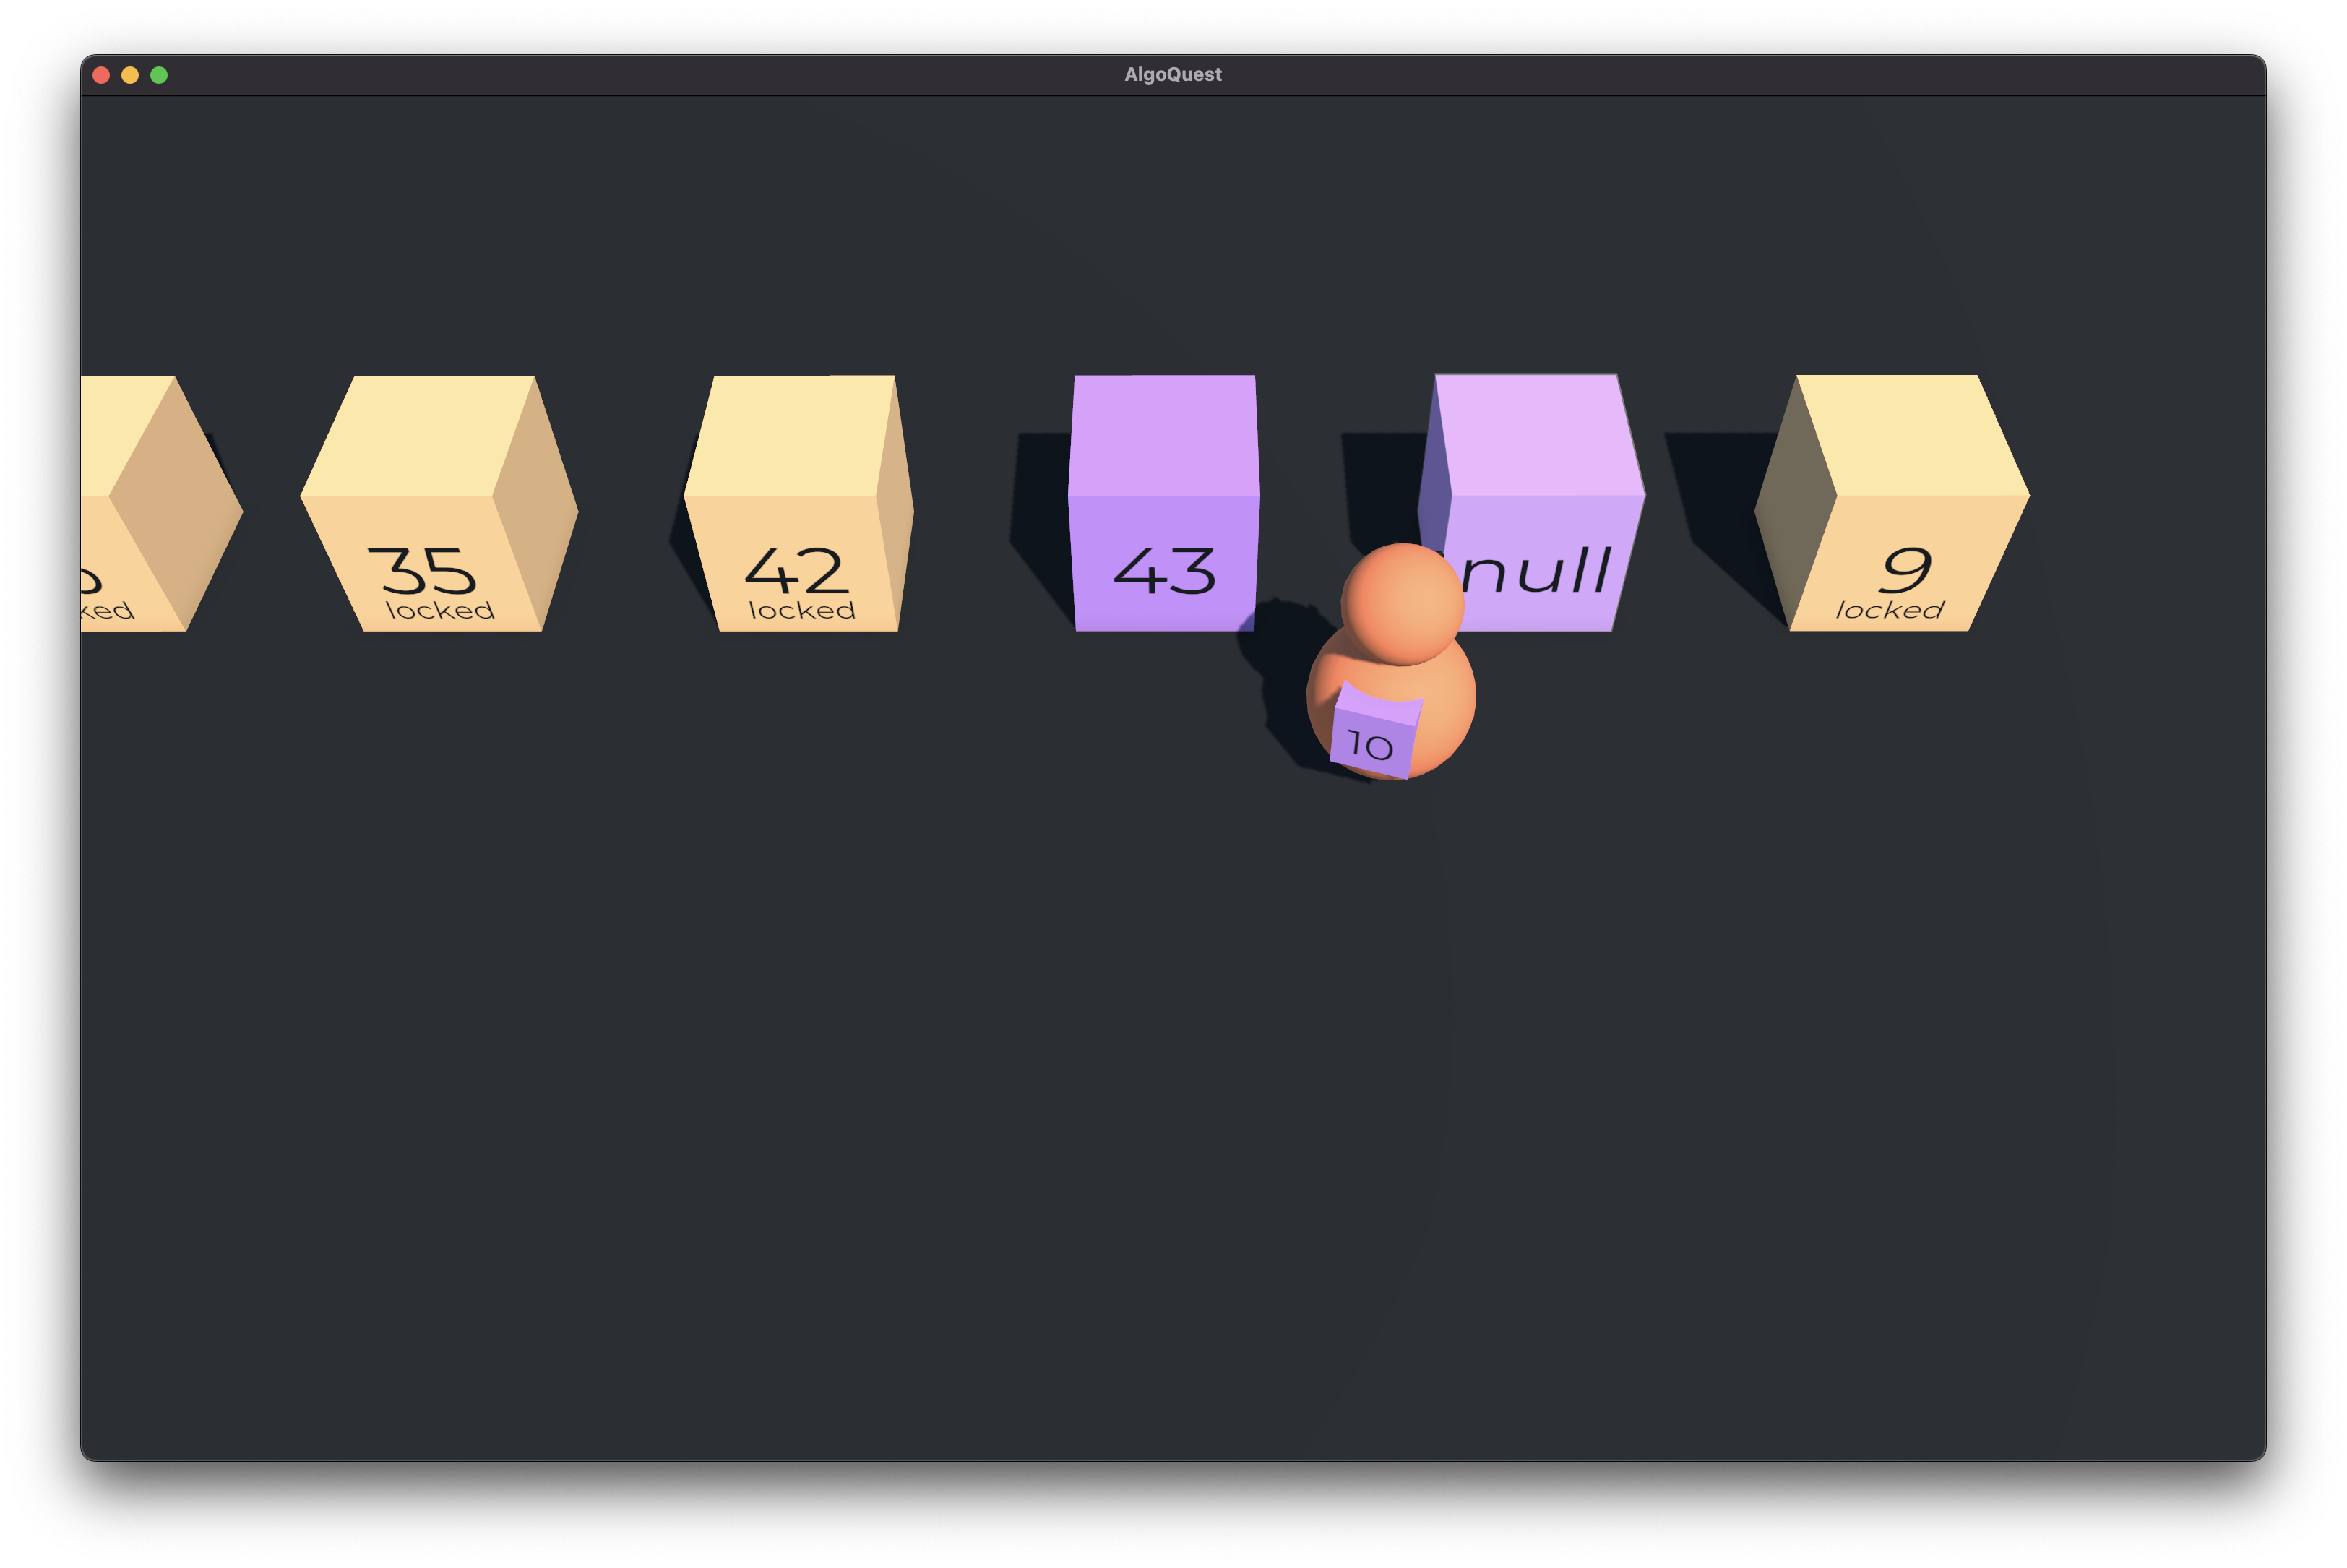
\includegraphics[width=0.7\linewidth]{sections/4/3/images/game_container_states}
    \caption{Οι τρεις καταστάσεις των κουτιών τιμών: \textbf{άδειο}(μωβ, \gls{null}), \textbf{γεμάτο}(μωβ, αριθμός) και \textbf{κλειδωμένο}(κίτρινο, αριθμός)}
    \label{fig:game_container_states}
\end{figure}

Στη κατάσταση \textbf{άδειο}, δεν περιέχουν καμία τιμή και περιμένουν κάποια τιμή να εισαχθεί από τον παίκτη. Εμφανίζουν την τιμή \gls{null}, στον παίκτη ως ένδειξη πως δεν περιέχουν καμία τιμή. Ο χρήστης αλληλεπιδρώντας με ένα τέτοιο κουτί, τοποθετεί την τιμή που μεταφέρει σε αυτό.

Στην κατάσταση \textbf{γεμάτο}, περιέχουν μία τυχαία δημιουργημένη τιμή και την εμφανίζουν στο χρήστη. Ο χρήστης αλληλεπιδρώντας με ένα τέτοιο κουτί, μπορεί είτε να πάρει την τιμή του εφόσον ο ίδιος δεν μεταφέρει κάποια άλλη τιμή, είτε να αλλάξει την τιμή που μεταφέρει με αυτή μέσα στο κουτί.

Η κατάσταση \textbf{κλειδωμένο} είναι μία ειδική περίπτωση που εμφανίζεται μόνο στη βοηθητική ροή και έχει ως σκοπό να καθοδηγήσει τον παίκτη να εκτελέσει τα σωστά βήματα στον αλγόριθμο. Οποιεσδήποτε αλληλεπιδράσεις με αυτά τα κουτιά είναι απενεργοποιημένες. Ένα κλειδωμένο κουτί έχει εμφανώς διαφορετικό χρώμα και ενημερώνει τον παίκτη για την κατάσταση του. Παρότι τα κουτιά είναι κλειδωμένα, οι τιμές που περιέχουν παραμένουν εμφανές στον παίκτη. Αυτό συμβαίνει διότι ο παίκτης πρέπει να μπορεί να δει όλες τις τιμές για να κατανοήσει τον λόγο για τον οποίο οι κινήσεις που επιτρέπονται είναι οι σωστές.

% ========================================

\subsubsection{Παίκτης}

Ο παίκτης, με το χαρακτηριστικό του σχήμα, έχει ένα κουτί το οποίο αναγράφει την τιμή που μεταφέρει ανά πάσα στιγμή. Σε αντίθεση με τα υπόλοιπα κουτιά, αυτό μπορεί να βρίσκεται είτε στη κατάσταση \textbf{άδειο} είτε \textbf{γεμάτο} και όχι κλειδωμένο. Μπορεί να κινηθεί στον χώρο ελεύθερα και είτε να πάρει μία τιμή από ένα κουτί είτε να αφήσει αυτήν που μεταφέρει. Στη περίπτωση που και το κουτί και ο παίκτης έχουν μία τιμή, τότε κατά την αλληλεπίδραση, αυτές εναλλάσσονται.

\begin{figure}[H]
    \centering
    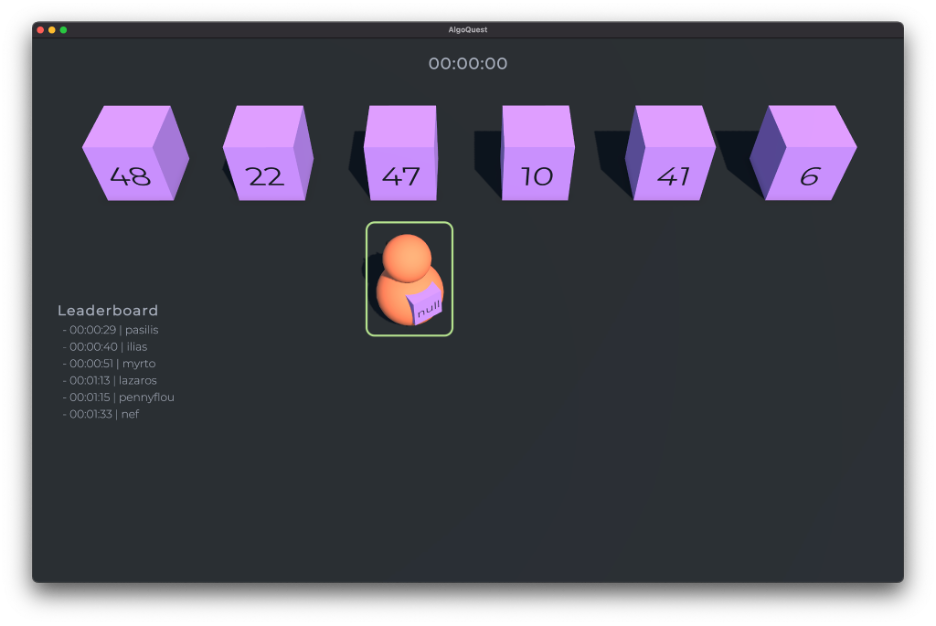
\includegraphics[width=0.8\linewidth]{sections/4/3/images/game_player}
    \caption{Ο παίκτης στο παιχνίδι}
    \label{fig:game_player}
\end{figure}
